\documentclass{beamer}
%
% Choose how your presentation looks.
%
% For more themes, color themes and font themes, see:
% http://deic.uab.es/~iblanes/beamer_gallery/index_by_theme.html
%
\mode<presentation>
{
  \usetheme{default}      % or try Darmstadt, Madrid, Warsaw, ...
  \usecolortheme{default} % or try albatross, beaver, crane, ...
  \usefonttheme{default}  % or try serif, structurebold, ...
  \setbeamertemplate{navigation symbols}{}
  \setbeamertemplate{caption}[numbered]
} 

\usepackage[english]{babel}
\usepackage[utf8x]{inputenc}
\usepackage{listings}
\usepackage{tabularx}
\usepackage{multirow}
\usepackage{booktabs}
\usepackage{tikz}

\title[]{Version Control Tool: Git}
\author{Biao Wang}
\institute{Anacode}
\date{\today}

\begin{document}

% \begin{frame}
%   \titlepage
% \end{frame}

% Uncomment these lines for an automatically generated outline.
\begin{frame}{Outline}
 \tableofcontents
\end{frame}

\section{Introduction}
\begin{frame}{Introduction}
    \begin{itemize}
      \item make your work organized      
    \end{itemize}  
    \begin{figure}
      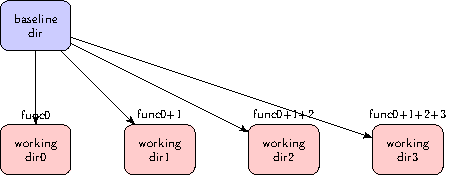
\includegraphics[width=.7\textwidth]{figures/withoutversioncontrol.pdf}      
    \end{figure}
    \begin{figure}
      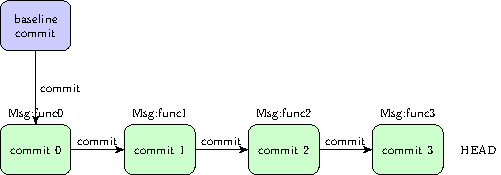
\includegraphics[width=.7\textwidth]{figures/withversioncontrol.pdf}
      \caption{\label{git life cycle} without and with version control.}
    \end{figure}         
\end{frame}

\begin{frame}{Introduction}
    \begin{itemize}
      \item debug your code
        \begin{itemize}
            \item make your life easy by narrowing down the problemetic code      
            \item But..., every commit shoud be verified before commit        
        \end{itemize}          
        \begin{figure}
        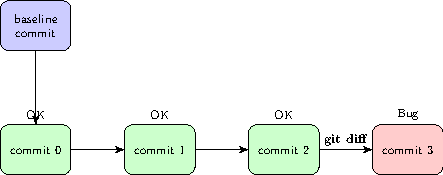
\includegraphics[width=.7\textwidth]{figures/debugversioncontrol.pdf}
        \end{figure}         
     \item teamwork development
        \begin{itemize}
            \item without version control tool, code management become extremely difficult.
        \end{itemize}          
    \end{itemize} 
\end{frame}

\section{Understanding git}
\begin{frame}{Understanding git: file status within git}
    \begin{figure}
    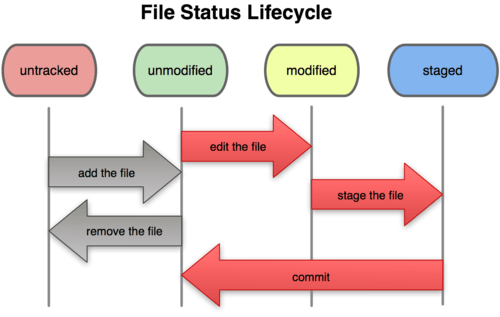
\includegraphics[width=.7\textwidth]{figures/gitlifestyle.png}
    \caption{\label{git life cycle} source: Internet.}
    \end{figure}             
\end{frame}

\begin{frame}{Understanding git: file status within git}
    Demo: how file status changes
    \begin{itemize}
     \item    add file: \textbf{git add          }
     \item modify file: \textbf{                 }
     \item  stage file: \textbf{git add (-u)     }
     \item commit file: \textbf{git commit -m ``Msg for this commit''}
     \begin{itemize}
        \item bad commit message: ``fix some bugs''
        \item would be better: ``fix SIMD memory load bugs within deblockingfilter.cpp''
     \end{itemize}
     \item remove file: \textbf{git rm       }
    \end{itemize}
    other useful commands: 
     \begin{itemize}
        \item git log:
	      \begin{itemize}
	       \item git log -\textit{n}: show the last \textbf{n} commit information
	       \item git log \textit{path}: show the last commit information regarding \textbf{path}
	      \end{itemize}
	\item git diff: show difference 	
     \end{itemize}    
\end{frame}

\begin{frame}{Understanding git: git diff}
    \begin{figure}
    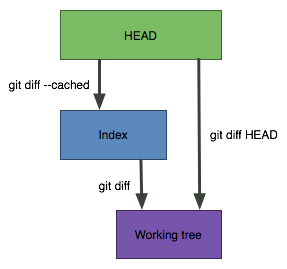
\includegraphics[width=.5\textwidth]{figures/GitDiffSimple.png}
    \caption{\label{git diff} source: Internet.}
    \end{figure}             
    \begin{itemize}
     \item    git diff: between the working directory and the index(staged)
     \item    git diff --cached: between the the index(staged) and HEAD
     \item    git diff HEAD: between the working directory and HEAD, includes changes in the index
    \end{itemize}
\end{frame}

\section{git in teamwork}
\begin{frame}{How to use git under team development senario}
    \begin{itemize}
      \item    git pull: to get the lastest copy of code.
      \item    git commit: commit your local code
      \item    git push: push your code change to the remote server
    \end{itemize}
    However, there might be a problem when you push
    \begin{figure}
      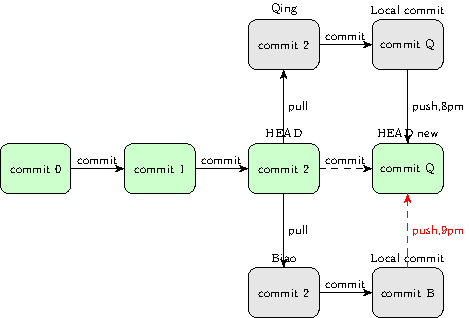
\includegraphics[width=.7\textwidth]{figures/withversioncontrolHead.pdf} 
      \caption{\label{git life cycle} team development using git.}
    \end{figure}    

\end{frame}

\begin{frame}{solution: prevent it happen}

    \begin{block}{Simple way}
      \begin{itemize}
	\item    git pull: to get the latest copy of code.
	\item    \textbf{before you commit, git pull again to make sure you are up-to-date}
	\item    git commit: commit your local code
	\item    git push: push your code change to the remote server
      \end{itemize}     
    \end{block}    
     
\end{frame}

\begin{frame}{solution: if you already commit}
    \begin{block}{Harder way: }
      \begin{itemize}      
	\item    git diff HEAD$\sim$1 $>$ yourcommit.diff : save your work into patch
	\item    git reset --hard HEAD$\sim$1: reset your code to HEAD(not commit B)
	\item    git pull: to get the latest copy of code (the HEAD new)
	\item    patch -p1 $<$ yourcommit.diff: apply patch
	\item    git add -u: add to the stage	
	\item    git commit: commit your local code
	\item    git push: push your code change to the remote server(create a node whose parent commit is HEAD new)
      \end{itemize}     
    \end{block}
\end{frame}

\section{Summary}

\begin{frame}{Summary}
    \begin{block}{work with git more effectively}
      \begin{itemize}      
	\item    file status: untracked, tracked, staged, commit
	\item    commands to change th status of file:
		\begin{itemize}      
		  \item git init
		  \item git add
		  \item git add -u
		  \item git commit 
		  \item git rm
		\end{itemize}     
	\item    working with other developers:
		\begin{itemize}      
		  \item use git pull frequently to make sure you are up-to-date
		  \item otherwise use git reset to go back to previous common parent commit, and apply patch
		\end{itemize}     	
      \end{itemize}     
    \end{block}
\end{frame}

\end{document}
